\documentclass{article}

% ------------------ Packages ------------------
\usepackage{graphicx}
\usepackage{amsmath}
\usepackage{amssymb}
\usepackage[margin=1in]{geometry}
\usepackage{xcolor}
\usepackage{tikz}
\usetikzlibrary{shapes,arrows.meta,positioning,calc,fit}
\usepackage{tcolorbox}
\usepackage{listings}

% ------------------ Code listing theme ------------------
\definecolor{codegreen}{rgb}{0,0.6,0}
\definecolor{codegray}{rgb}{0.5,0.5,0.5}
\definecolor{codepurple}{rgb}{0.58,0,0.82}
\definecolor{backcolour}{rgb}{0.95,0.95,0.92}

\lstdefinestyle{pythonstyle}{
    backgroundcolor=\color{backcolour},
    commentstyle=\color{codegreen},
    keywordstyle=\color{magenta},
    numberstyle=\tiny\color{codegray},
    stringstyle=\color{codepurple},
    basicstyle=\ttfamily\footnotesize,
    breaklines=true,
    captionpos=b,
    keepspaces=true,
    numbers=left,
    numbersep=6pt,
    showspaces=false,
    showstringspaces=false,
    showtabs=false,
    tabsize=2
}
\lstset{style=pythonstyle}

% ------------------ Unified TikZ legend (Colah-style) ------------------
% Palette
\definecolor{colahPink}{RGB}{255,155,170}    % pointwise ops (×, +)
\definecolor{colahYellow}{RGB}{255,230,128}  % learned gates/layers (σ, tanh)
\definecolor{colahBlue}{RGB}{190,220,255}    % states (h, C) and modules
\definecolor{colahGray}{gray}{0.25}          % stroke

% Styles (consistent across all figures)
\tikzset{
  >=Latex,
  flow/.style       = {-Latex, thick, shorten >=1pt, shorten <=1pt},
  dashedflow/.style = {-Latex, thick, dashed, shorten >=1pt, shorten <=1pt},
  op/.style         = {circle, draw=colahGray, fill=colahPink!70,
                       inner sep=0pt, minimum size=6mm, font=\small},
  subop/.style      = {circle, draw=colahGray, fill=colahPink!70,
                       inner sep=0pt, minimum size=4mm, font=\tiny},
  layer/.style      = {rectangle, draw=colahGray, rounded corners=2pt, fill=colahYellow!70,
                       minimum width=1.8cm, minimum height=8mm, align=center},
  statebox/.style   = {rectangle, draw=colahGray, rounded corners=2pt, fill=colahBlue!45,
                       minimum height=8mm, align=center},
  data/.style       = {rectangle, draw=colahGray, rounded corners=2pt, fill=orange!30,
                       minimum height=8mm, align=center},
  note/.style       = {font=\scriptsize, inner sep=1pt}
}

% A tiny grid helper for consistent y-levels in all cell diagrams
\newcommand{\yCell}{2}      % cell-state rail
\newcommand{\yHid}{0}       % hidden/output rail
\newcommand{\yInp}{-1.2}    % input rail

% ------------------ Document meta ------------------
\title{Lecture 7 RNNs and Gated Architectures\\
\large From Fixed Representations to Sequential Memory}
\author{Deep Learning Class}
\date{\today}

\begin{document}
\maketitle

% % ====================================================
% \section{Opening: The Evolution Continues}

% Last time, we built autoencoders—the encoder–decoder framework that compresses any input to a fixed-size representation. But we hit a wall: \emph{long sequences}! A sentence can be 5 words or 500 words. A song can be 3 minutes or 30 minutes. Today, we tackle this challenge head-on.

% \begin{tcolorbox}[colback=blue!5!white, colframe=blue!60!black, title=Our Journey So Far]
% \textbf{Lecture 6:} Autoencoders $\rightarrow$ Fixed-size bottleneck for any input
% \textbf{Today:} RNNs $\rightarrow$ Process sequences step by step

% \begin{itemize}
% \item \emph{Why a (seq2seq) AE is not sufficient?} A single fixed-length code $z\in\mathbb{R}^d$ must summarize a $T$-step input. Information-theoretically, $I(x_{1:T};z)\le H(z)=\mathcal{O}(d)$, so the \emph{per-token} capacity $I(x_{1:T};z)/T\to 0$ as $T\to\infty$. Long-range dependencies get squeezed through a narrow bottleneck.
% \item \emph{Avoiding fixed-size padding.} Making the AE accept length-$L$ inputs by padding short sequences ($x_t=\mathrm{PAD}$ for $t>T$) wastes compute $\mathcal{O}(L-T)$, leaks position cues (the model learns ``where real data stops''), and biases statistics/training dynamics.
% \item \emph{Streaming constraint.} For a live stream $(x_t)_{t\ge1}$, an AE requires a full window to encode. RNNs maintain a finite \emph{state} that updates online.
% enabling constant-memory, stepwise ingestion without waiting for the entire sequence.
% \end{itemize}

% \textbf{Coming Soon:} Transformers $\rightarrow$ Process all steps in parallel
% \emph{Bridge:} RNNs provide the stateful, causal view; Transformers remove recurrence and use self-attention to create short paths across time while adding positional structure. This lecture sets up that transition.
% \end{tcolorbox}

% ====================================================

\section{Why RNNs? The Failure of Seq2Seq Autoencoders}

\subsection{The Tempting Autoencoder Approach}

Coming from Lecture 6, you might think: ``Why not just use an autoencoder for sequences?'' For translation, we could:

\begin{center}
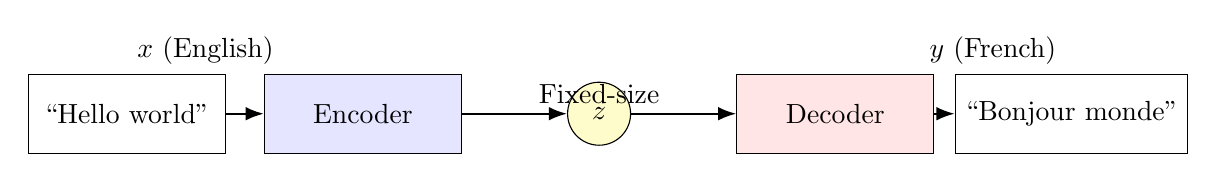
\begin{tikzpicture}[
    box/.style={rectangle, draw, minimum width=2.5cm, minimum height=1cm},
    latent/.style={circle, draw, fill=yellow!20, minimum size=0.8cm},
    arrow/.style={->, thick}
]
% English sentence
\node[box] (input) at (0,0) {``Hello world''};
\node[box, fill=blue!10] (encoder) at (3,0) {Encoder};
\node[latent] (z) at (6,0) {$z$};
\node[box, fill=red!10] (decoder) at (9,0) {Decoder};
\node[box] (output) at (12,0) {``Bonjour monde''};

% Arrows
\draw[arrow] (input) -- (encoder);
\draw[arrow] (encoder) -- (z);
\draw[arrow] (z) -- (decoder);
\draw[arrow] (decoder) -- (output);

% Labels
\node[above] at (1,.5) {$x$ (English)};
\node[above] at (11,0.5) {$y$ (French)};
\node[above] at (z) {Fixed-size};
\end{tikzpicture}
 \end{center}

This looks elegant! But it catastrophically fails for real sequences. Let's understand why.

\subsection{Problem 1: The Information Bottleneck Disaster}

\begin{tcolorbox}[colback=red!5!white, colframe=red!50!black, title=The Bottleneck Mathematics]
Consider encoding sequences of varying lengths into a fixed-size latent $z \in \mathbb{R}^d$:

\begin{itemize}
\item 5-word tweet: ``Great weather today in Paris'' $\rightarrow$ $z \in \mathbb{R}^{128}$
\item 500-word essay: [entire paragraph] $\rightarrow$ $z \in \mathbb{R}^{128}$
\item 50,000-word novel: [entire book] $\rightarrow$ $z \in \mathbb{R}^{128}$
\end{itemize}

Information-theoretically, the mutual information is bounded:
$$I(x_{1:T}; z) \leq H(z) \approx d \log 2$$

As $T \rightarrow \infty$, the per-token information capacity:
$$\frac{I(x_{1:T}; z)}{T} \rightarrow 0$$

\textbf{Result:} You're trying to compress ``War and Peace'' into the same space as a text message!
\end{tcolorbox}

\subsection{Problem 2: Lack of Sequential Structure}

Autoencoders treat input as a ``bag of features''—they don't naturally preserve order:

\begin{center}
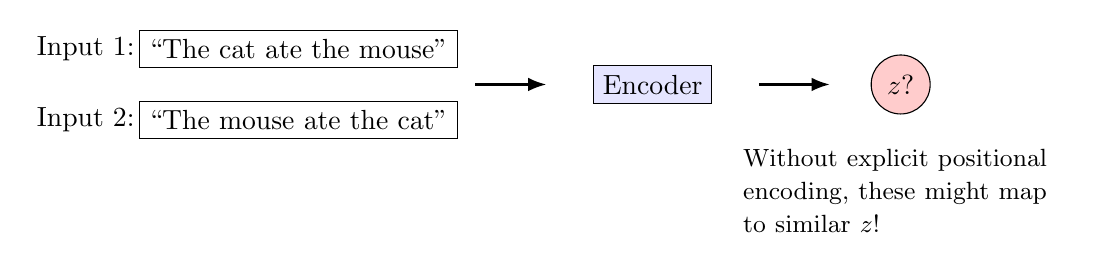
\begin{tikzpicture}[scale=0.9]
% Original sentence
\node at (0, 2) {Input 1:};
\node[draw, rectangle] at (3, 2) {``The cat ate the mouse''};

\node at (0, 1) {Input 2:};
\node[draw, rectangle] at (3, 1) {``The mouse ate the cat''};

% Arrow to encoder
\draw[->, thick] (5.5, 1.5) -- (6.5, 1.5);

% Encoder box
\node[draw, rectangle, fill=blue!10] at (8, 1.5) {Encoder};

% Arrow to same latent
\draw[->, thick] (9.5, 1.5) -- (10.5, 1.5);

% Same latent representation!
\node[draw, circle, fill=red!20] at (11.5, 1.5) {$z$?};

\node[text width=4cm] at (11.5, 0) {\small Without explicit positional encoding, these might map to similar $z$!};
\end{tikzpicture}
\end{center}

Order matters in language! ``Dog bites man'' $\neq$ ``Man bites dog''.

\subsection{Problem 3: The Variable-Length Nightmare}

Real sequences have wildly different lengths. Autoencoders require fixed-size inputs, leading to ugly hacks:

\begin{tcolorbox}[colback=yellow!5!white, colframe=orange!50!black, title=The Padding Problem]
To handle variable lengths in autoencoders, we must either:

\textbf{Option A: Pad to maximum length}
\begin{lstlisting}[language=Python]
# Waste computation on padding tokens
x1 = ["Hello", ``world", ``PAD", ``PAD", ..., ``PAD"]  # 5% real data
x2 = ["The", ``quick", ``brown", ..., ``jumped"]      # 100% real data
\end{lstlisting}

Problems:
\begin{itemize}
\item Wastes $O(L_{\text{max}} - L_{\text{actual}})$ computation
\item Model learns spurious patterns about where ``real data ends''
\item Batch efficiency destroyed by outliers
\end{itemize}

\textbf{Option B: Truncate to fixed length}
\begin{lstlisting}[language=Python]
# Throw away information!
x_long = text[:MAX_LENGTH]  # Lose everything after position 512
\end{lstlisting}

Problems:
\begin{itemize}
\item Information loss
\item Can't handle naturally long sequences (documents, conversations)
\end{itemize}
\end{tcolorbox}

\subsection{Problem 4: No Natural Chunking or Streaming}

Autoencoders need the \textbf{entire sequence} before encoding:

\begin{center}
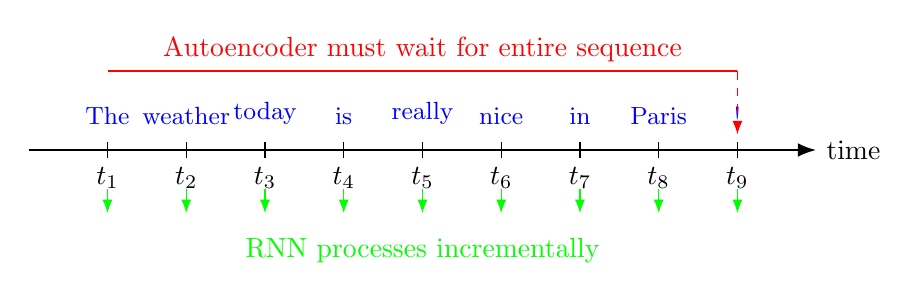
\begin{tikzpicture}
% Timeline
\draw[thick, ->] (0,0) -- (10,0) node[right] {time};
\foreach \x in {1,2,3,4,5,6,7,8,9} {
    \draw (\x, -0.1) -- (\x, 0.1);
    \node[below] at (\x, -0.1) {$t_\x$};
}

% Words arriving
\foreach \x/\word in {1/The, 2/weather, 3/today, 4/is, 5/really, 6/nice, 7/in, 8/Paris, 9/!} {
    \node[above, blue] at (\x, 0.2) {\small \word};
}

% Autoencoder waits
\draw[red, thick] (1, 1) -- (9, 1);
\node[red, above] at (5, 1) {Autoencoder must wait for entire sequence};
\draw[red, dashed, ->] (9, 1) -- (9, 0.2);

% RNN processes incrementally
\foreach \x in {1,2,3,4,5,6,7,8,9} {
    \draw[green, ->] (\x, -0.5) -- (\x, -0.8);
}
\node[green, below] at (5, -1) {RNN processes incrementally};
\end{tikzpicture}
\end{center}

This makes autoencoders impossible for:
\begin{itemize}
\item Live transcription/translation
\item Streaming data analysis
\item Interactive chatbots
\item Any real-time application
\end{itemize}


\section{Module 2: RNNs - The Stateful Summarizer}

We now transition from static data to sequence data ($X_1, X_2, ..., X_T$). Our goal is to maintain an understanding of the sequence over time.

\subsection{The Naive Approach: Unrolled MLPs}

Let's try using an MLP at each time step. We process the input $X_t$ at time $t$ to get a hidden representation $H_t$.

\begin{enumerate}
    \item \textbf{Initial thought:} $H_t = \text{Embed}(X_t)$. This has no memory.
    \item \textbf{Adding memory:} To understand the sequence, the state at time $t$ must know about the state at time $t-1$. We introduce a connection:
    $$H_t = f_t(H_{t-1}, X_t)$$
\end{enumerate}

\begin{center}
    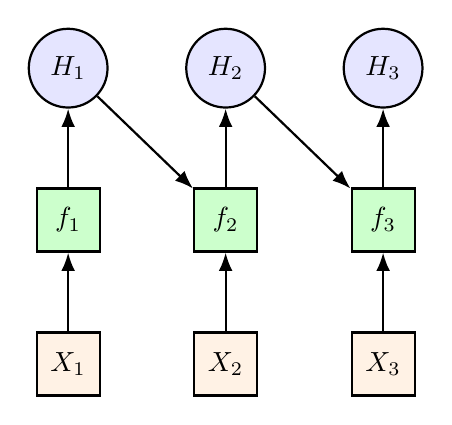
\begin{tikzpicture}[
        node distance=2cm,
        state/.style={circle, draw, minimum size=1cm, thick, fill=blue!10},
        input/.style={rectangle, draw, minimum size=0.8cm, thick, fill=orange!10},
        func/.style={rectangle, draw, minimum size=0.8cm, thick, fill=green!20},
        arrow/.style={->, thick}
    ]
        % Inputs
        \node[input] (x1) {$X_1$};
        \node[input, right of=x1] (x2) {$X_2$};
        \node[input, right of=x2] (x3) {$X_3$};
        
        % Functions
        \node[func, above=1cm of x1] (f1) {$f_1$};
        \node[func, above=1cm of x2] (f2) {$f_2$};
        \node[func, above=1cm of x3] (f3) {$f_3$};

        % Hidden states
        \node[state, above=1cm of f1] (h1) {$H_1$};
        \node[state, above=1cm of f2] (h2) {$H_2$};
        \node[state, above=1cm of f3] (h3) {$H_3$};
        
        % Connections
        \draw[arrow] (x1) -- (f1);
        \draw[arrow] (x2) -- (f2);
        \draw[arrow] (x3) -- (f3);
        \draw[arrow] (f1) -- (h1);
        \draw[arrow] (f2) -- (h2);
        \draw[arrow] (f3) -- (h3);

        \draw[arrow] (h1) -- (f2);
        \draw[arrow] (h2) -- (f3);
        
    \end{tikzpicture}
    \textit{Visualization of the unrolled network with time-variant functions $f_t$.}
\end{center}

\subsubsection{The Failure of the Naive Approach}

This ``unrolled MLP'' approach, using a time-variant $f_t$, has critical flaws:

\begin{itemize}
    \item \textbf{Problem 1: Parameter Explosion.} The weights for $f_1$ are different from $f_2$, $f_3$, etc. The number of parameters grows linearly with the sequence length $T$.
    \item \textbf{Problem 2: Lack of Generalization (Stationarity).} The model assumes the rules governing the sequence (e.g., grammar or physics) change at every time step. It cannot generalize knowledge learned at $T=1$ to $T=100$.
\end{itemize}

\subsection{The Key Innovation: Recurrence (Parameter Sharing)}

What if we enforce stationarity? We force the network to use the \textit{exact same function} at every single time step. This is analogous to how CNNs share parameters (filters) across space.

We move from $H_t = f_t(H_{t-1}, X_t)$ to:
$$ \mathbf{H_t = f(H_{t-1}, X_t)} $$

This is the definition of a Recurrent Neural Network (RNN). The model size is now independent of the sequence length.

\begin{center}
    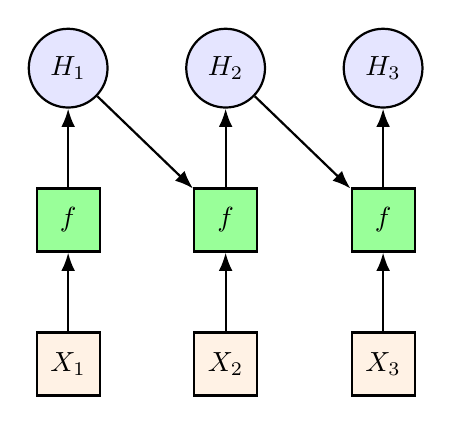
\begin{tikzpicture}[
        node distance=2cm,
        state/.style={circle, draw, minimum size=1cm, thick, fill=blue!10},
        input/.style={rectangle, draw, minimum size=0.8cm, thick, fill=orange!10},
        func/.style={rectangle, draw, minimum size=0.8cm, thick, fill=green!40},
        arrow/.style={->, thick}
    ]
        % Inputs
        \node[input] (x1) {$X_1$};
        \node[input, right of=x1] (x2) {$X_2$};
        \node[input, right of=x2] (x3) {$X_3$};
        
        % Functions (Now the same 'f')
        \node[func, above=1cm of x1] (f1) {$f$};
        \node[func, above=1cm of x2] (f2) {$f$};
        \node[func, above=1cm of x3] (f3) {$f$};

        % Hidden states
        \node[state, above=1cm of f1] (h1) {$H_1$};
        \node[state, above=1cm of f2] (h2) {$H_2$};
        \node[state, above=1cm of f3] (h3) {$H_3$};
        
        % Connections
        \draw[arrow] (x1) -- (f1);
        \draw[arrow] (x2) -- (f2);
        \draw[arrow] (x3) -- (f3);
        \draw[arrow] (f1) -- (h1);
        \draw[arrow] (f2) -- (h2);
        \draw[arrow] (f3) -- (h3);

        \draw[arrow] (h1) -- (f2);
        \draw[arrow] (h2) -- (f3);
        
    \end{tikzpicture}
    \textit{The RNN architecture: the same function $f$ is applied at every time step.}
\end{center}



\subsubsection{The Hidden State as Memory (The Markovian Concept)}

Because the same function $f$ is applied repeatedly, $H_t$ must act as a distilled summary of the entire history ($X_1, ..., X_t$). This derives the Markovian representation of a dynamical system in the hidden state: given $H_t$, we (ideally) don't need any info from the past, as we have all we need distilled into the state $H_t$.

\subsection{The Basic (Vanilla) RNN Architecture}

Mathematically, the vanilla RNN is defined as:

$$\mathbf{h}_t = \tanh(\mathbf{W}_{xh} \mathbf{x}_t + \mathbf{W}_{hh} \mathbf{h}_{t-1} + \mathbf{b}_h)$$

Where $\mathbf{W}_{hh}$ is the recurrent weight matrix.

\subsection{So RNN solves the problems in AE}

So RNNs solve the AE problems through their fundamental design:

\begin{center}
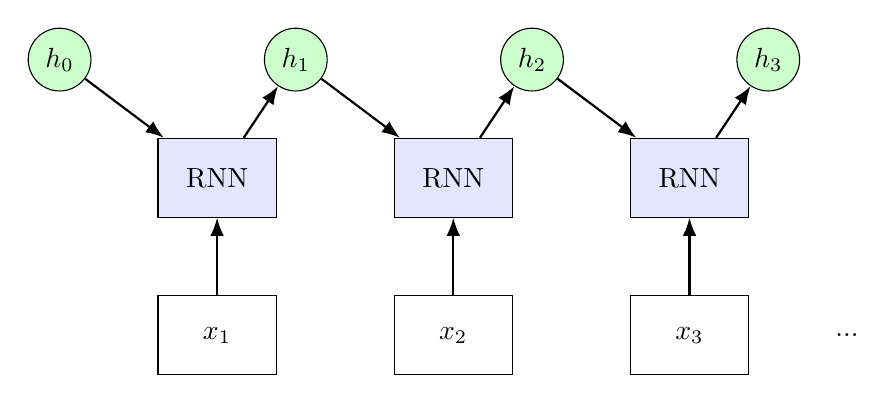
\begin{tikzpicture}[
    node distance=1cm,
    box/.style={rectangle, draw, minimum width=1.5cm, minimum height=1cm},
    state/.style={circle, draw, fill=green!20},
    arrow/.style={->, thick}
]
% Time steps
\node[box] (x1) at (0,-1) {$x_1$};
\node[box] (x2) at (3,-1) {$x_2$};
\node[box] (x3) at (6,-1) {$x_3$};
\node at (8,-1) {...};

% Hidden states
\node[state] (h0) at (-2,2.5) {$h_0$};
\node[state] (h1) at (1,2.5) {$h_1$};
\node[state] (h2) at (4,2.5) {$h_2$};
\node[state] (h3) at (7,2.5) {$h_3$};

% RNN cells
\node[box, fill=blue!10] (f1) at (0,1) {RNN};
\node[box, fill=blue!10] (f2) at (3,1) {RNN};
\node[box, fill=blue!10] (f3) at (6,1) {RNN};

% Connections
\draw[arrow] (h0) -- (f1);
\draw[arrow] (x1) -- (f1);
\draw[arrow] (f1) -- (h1);

\draw[arrow] (h1) -- (f2);
\draw[arrow] (x2) -- (f2);
\draw[arrow] (f2) -- (h2);

\draw[arrow] (h2) -- (f3);
\draw[arrow] (x3) -- (f3);
\draw[arrow] (f3) -- (h3);
\end{tikzpicture}
\end{center}

\begin{tcolorbox}[colback=green!5!white, colframe=green!50!black, title=Why RNNs Win]
\textbf{1. No one time compression, instead information accumulation:} Information accumulates in the hidden state $h_t$ rather than being compressed all at once.

\textbf{2. Natural ordering:} Sequential processing inherently preserves temporal structure.

\textbf{3. Variable length handling:} Process sequences of any length with the same model—no padding needed!

\textbf{4. Streaming capability:} Process data as it arrives, maintaining state between time steps.

\textbf{5. Computational efficiency:} $O(T)$ memory and computation, not $O(T^2)$ or $O(L_{\text{max}})$.

\textbf{6. Parameter sharing:} Same function at each step $\rightarrow$ model size independent of sequence length.
\end{tcolorbox}

\subsection{Case Study: Machine Translation}

Let's see why the autoencoder fails and RNN succeeds for translation:

\begin{center}
\textbf{Autoencoder Approach (Fails):}
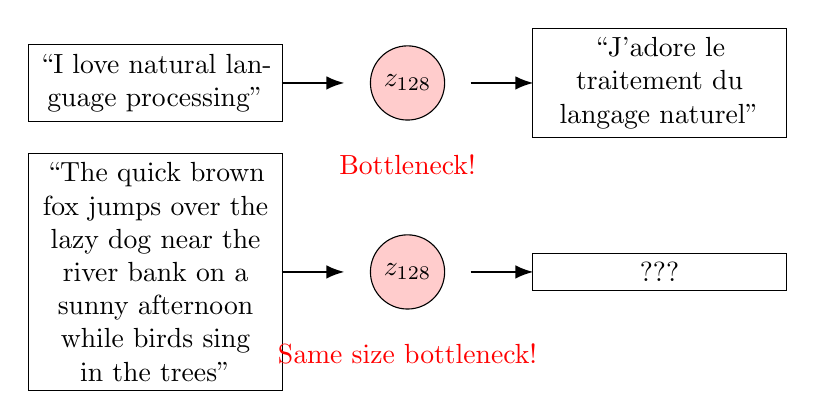
\begin{tikzpicture}[scale=0.8]
% English sentence of varying length
\node[draw, text width=3cm, align=center] (eng) at (0,0) {``I love natural language processing''};
\draw[->, thick] (2,0) -- (3,0);
\node[draw, circle, fill=red!20] (z) at (4,0) {$z_{128}$};
\draw[->, thick] (5,0) -- (6,0);
\node[draw, text width=3cm, align=center] (fr) at (8,0) {``J'adore le traitement du langage naturel''};

\node[below, red] at (4,-1) {Bottleneck!};

% Longer sentence
\node[draw, text width=3cm, align=center] (eng2) at (0,-3) {``The quick brown fox jumps over the lazy dog near the river bank on a sunny afternoon while birds sing in the trees''};
\draw[->, thick] (2,-3) -- (3,-3);
\node[draw, circle, fill=red!20] (z2) at (4,-3) {$z_{128}$};
\draw[->, thick] (5,-3) -- (6,-3);
\node[draw, text width=3cm, align=center] (fr2) at (8,-3) {???};

\node[below, red] at (4,-4) {Same size bottleneck!};
\end{tikzpicture}
\end{center}

\begin{center}
\textbf{RNN Approach (Works):}
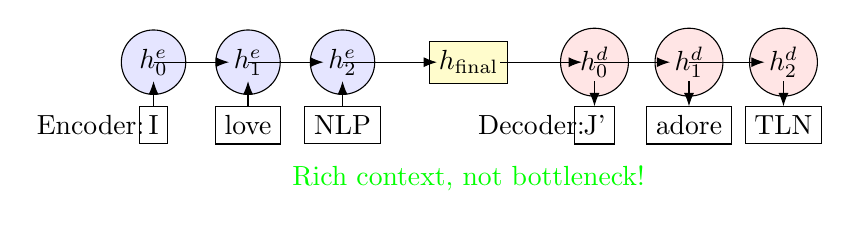
\begin{tikzpicture}[scale=0.8]
% Encoder RNN
\node at (-1, 0) {Encoder:};
\foreach \x/\word in {0/I, 1/love, 2/NLP} {
    \node[draw, rectangle] at (\x*1.5, 0) {\word};
    \node[draw, circle, fill=blue!10] at (\x*1.5, 1) {$h_\x^e$};
    \draw[->] (\x*1.5, 0.3) -- (\x*1.5, 0.7);
}
\draw[->] (0, 1) -- (1.2, 1);
\draw[->] (1.5, 1) -- (2.7, 1);

% Context vector (final hidden state)
\node[draw, rectangle, fill=yellow!20] at (5, 1) {$h_{\text{final}}$};
\draw[->] (3, 1) -- (4.5, 1);

% Decoder RNN
\node at (6, 0) {Decoder:};
\foreach \x/\word in {0/J', 1/adore, 2/TLN} {
    \node[draw, rectangle] at (7+\x*1.5, 0) {\word};
    \node[draw, circle, fill=red!10] at (7+\x*1.5, 1) {$h_\x^d$};
    \draw[->] (7+\x*1.5, 0.7) -- (7+\x*1.5, 0.3);
}
\draw[->] (5.5, 1) -- (6.8, 1);
\draw[->] (7, 1) -- (8.2, 1);
\draw[->] (8.5, 1) -- (9.7, 1);

\node[below, green] at (5, -0.5) {Rich context, not bottleneck!};
\end{tikzpicture}
\end{center}

The RNN encoder builds up a rich representation step-by-step, and the decoder unrolls it step-by-step. No fixed-size bottleneck!

\subsection{Summary: From Autoencoders to RNNs}

\begin{tabular}{|l|c|c|}
\hline
\textbf{Challenge} & \textbf{Autoencoder} & \textbf{RNN} \\
\hline
Variable-length sequences & Padding/Truncation & Native support \\
Information bottleneck & Fixed $z$ size & Evolving $h_t$ \\
Sequential structure & Must add position encoding & Built-in via recurrence \\
Streaming/Online processing & Impossible & Natural \\
Computational efficiency & $O(L_{\text{max}})$ always & $O(T_{\text{actual}})$ \\
Long sequences & Bottleneck collapse & Gradual processing \\
\hline
\end{tabular}

\textbf{The key insight:} Instead of compressing everything at once (autoencoder), we process and maintain state incrementally (RNN). This is why we need the recurrent structure!



\subsection{The Vanishing and Exploding Gradient Problem (VEGP)}

Training RNNs involves Backpropagation Through Time (BPTT). The gradient from time t back to time $t-k$ contains a product of Jacobians:

Thus,
\[
\frac{\partial \mathbf{h}_{t}}{\partial \mathbf{h}_{t-k}}=\prod_{j=t-k+1}^{t}\underbrace{\text{diag}(1-\tanh^{2}(\cdot))}_{\le I}W_{hh}.
\]
\[
||\frac{\partial \mathbf{h}_{t}}{\partial \mathbf{h}_{t-k}}||\le\prod_{j=1}^{k}||W_{hh}||\,||\text{diag}(1-\tanh^{2})||,
\]
so if the top singular value of $W_{hh}$ is $<1$, gradients vanish exponentially; if $>1$, they explode.

\begin{tcolorbox}[colback=red!5!white,colframe=red!60!black,title=The Severity of VEGP: A Numerical Intuition]
The core issue is the repeated multiplication by the recurrent weight $W_{hh}$. Vanilla RNNs use the same feedback loop connection for events that happened long ago and events that just happened.

To understand why this is catastrophic, consider a simplified view where the Jacobian essentially acts like the weight $W_{hh}$. If we unroll the network for just 50 steps (e.g., 50 days of stock data):
\begin{itemize}
    \item \textbf{Exploding Gradients:} If $||W_{hh}|| > 1$ (e.g., $W_{hh}=2$), the gradient is scaled by a factor related to $2^{50} \approx 1.12 \times 10^{15}$. The gradient explodes. Kaboom!
    \item \textbf{Vanishing Gradients:} If $||W_{hh}|| < 1$ (e.g., $W_{hh}=0.5$), the gradient is scaled by a factor related to $0.5^{50} \approx 8.88 \times 10^{-16}$. The gradient vanishes. Poof!
\end{itemize}
In either case, the network cannot effectively learn connections between events that are far apart in the sequence.
\end{tcolorbox}

Gradient clipping (band-aid).
\[
\mathbf{g}\leftarrow\min\left(1,\frac{\theta}{||\mathbf{g}||}\right)\mathbf{g}
\]
Vanishing gradients need architectural help: gates.



\subsection{Training RNNs: Backpropagation Through Time and Truncation Strategies}

\subsubsection{The Computational Challenge of Full BPTT}

While BPTT provides exact gradients, computing gradients across entire sequences is often computationally infeasible:

\begin{itemize}
\item \textbf{Memory explosion:} Storing all intermediate activations for a 1000-step sequence requires massive memory.
\item \textbf{Numerical instability:} As we've seen, gradients either vanish or explode over long sequences.
\item \textbf{Computational cost:} The gradient computation scales as $O(T^2)$ for sequence length $T$.
\end{itemize}

\subsubsection{Truncation Strategies}

To make RNN training practical, we truncate the backpropagation, limiting how far back gradients flow. Three main strategies exist:

% LICENSING OMISSION: the original lecture source embedded D2L Fig. 9.7.1 here.
% The third-party figure and its caption are intentionally excluded from this
% repository; retain only the independently written comparison below.


\begin{enumerate}
\item \textbf{Randomized Truncation:} Partition sequences into segments of varying lengths.
\item \textbf{Regular Truncation:} Break sequences into fixed-length subsequences (e.g., chunks of 35 steps).
\item \textbf{Full BPTT:} Process the entire sequence—computationally infeasible for long sequences.
\end{enumerate}

\subsubsection{Why Regular Truncation Wins in Practice}

Despite randomized truncation being theoretically unbiased, \textbf{regular truncation} is overwhelmingly preferred in practice. Here's why:

\begin{tcolorbox}[colback=green!5!white, colframe=green!50!black, title=The Three Pillars of Regular Truncation's Success]

\textbf{1. Far-past effects fade fast.} \\
After a modest number of steps (e.g., 20-50), the influence of a past observation on the current gradient is usually tiny due to:
\begin{itemize}
\item Vanishing gradients: $\|\partial h_t / \partial h_{t-k}\| \sim \|W_{hh}\|^k$ decays exponentially
\item Mixing dynamics: Information gets ``diluted'' as it passes through many nonlinearities
\end{itemize}
A fixed window already captures what matters; making it longer adds little signal.

\textbf{2. Variance vs. accuracy trade-off.} \\
Randomized truncation is unbiased in expectation, but introduces \textbf{higher gradient variance}:
\begin{itemize}
\item Different minibatches see wildly different truncation lengths
\item This noise cancels the theoretical benefit of ``occasionally'' using longer spans
\item Optimization tends to be worse than with a stable fixed window
\end{itemize}

\textbf{3. Useful inductive bias (``regularization'').} \\
We often \textit{want} models with a \textbf{short range of interactions}:
\begin{itemize}
\item Simpler models generalize better
\item More stable training dynamics
\item Regular truncation imposes this bias, acting like a mild regularizer
\item Prevents overfitting to spurious long-range correlations
\end{itemize}
\end{tcolorbox}

\subsubsection{Implementation: Detached State Carrying}

In practice, we implement regular truncation as follows:

\begin{lstlisting}[language=Python, caption=Regular Truncation with Detached State Carrying]
def train_rnn_truncated(model, data, chunk_size=35):
    ``""Train RNN with regular truncation."""
    hidden = model.init_hidden()  # Initialize h_0
    
    for epoch in range(num_epochs):
        for t in range(0, len(data), chunk_size):
            # Extract chunk
            chunk = data[t:t+chunk_size]
            
            # Forward pass with carried state
            outputs, new_hidden = model(chunk, hidden)
            
            # Compute loss
            loss = compute_loss(outputs, targets)
            
            # Backward pass (gradients only flow within chunk)
            loss.backward()
            
            # CRITICAL: Detach hidden state to stop gradient flow
            hidden = new_hidden.detach()  # Break gradient chain
            
            # Update weights
            optimizer.step()
\end{lstlisting}

The key insight: \texttt{hidden = new\_hidden.detach()} prevents gradients from flowing beyond chunk boundaries while still carrying the state information forward.

\begin{tcolorbox}[colback=yellow!5!white, colframe=orange!50!black, title=Practical Recommendations]
\begin{itemize}
\item \textbf{Chunk size:} Typically 20-100 steps (35 is common for character-level models)
\item \textbf{State initialization:} Zero or learned initial state
\item \textbf{Gradient clipping:} Essential! Clip to norm 5-10
\item \textbf{For very long sequences:} Consider hierarchical models or attention mechanisms
\end{itemize}
\end{tcolorbox}

\textbf{Summary:} Train on \textbf{fixed-length chunks}, keep your $x_t$, $h_t$, and $o_t$ aligned within each chunk, detach the carried state between chunks, and you'll get the practical sweet spot of efficiency, stability, and performance.


\bigskip

% 
% ====================================================
% Section 2.4.1 (Enhanced transition and content from previous turn)
% ====================================================

\section{From RNN to LSTM: a design-by-constraints story}

To address the limitations of vanilla RNNs, we introduce the Long Short-Term Memory (LSTM) architecture. The main idea is to decouple the memory into two separate pathways:
\begin{itemize}
    \item \textbf{Long-Term Memory (The Cell State, $\mathbf{C}_t$):} Designed to preserve information over many time steps by avoiding direct, repeated weight multiplication.
    \item \textbf{Short-Term Memory (The Hidden State, $\mathbf{h}_t$):} Designed as the ``working memory'' relevant to the current step, similar to a vanilla RNN state.
\end{itemize}

We now \emph{engineer} a recurrent cell that manages these two pathways while remaining writable, forgettable, and readable.

\begin{enumerate}
    \item \textbf{Preserve information additively.} We design the Long-Term Memory (Cell State $\mathbf{C}_t$) as a \textbf{conveyor belt}. We replace repeated nonlinear overwrites with an additive accumulator:
    $\mathbf{C}_t=\mathbf{C}_{t-1}+\Delta_t$. This allows information (and gradients) to flow largely unchanged, as there are no weights directly modifying the main pathway.
    
    \item \textbf{Control forgetting.} Introduce a Forget Gate $\mathbf{F}_t\in(0,1)$ that scales how much of the long-term memory survives: $\mathbf{C}_t=\mathbf{F}_t\odot\mathbf{C}_{t-1}+\cdots$.
    
    \item \textbf{Control writing.} Use an \emph{input gate} $\mathbf{I}_t$ and a candidate memory $\tilde{\mathbf{C}}_t$ to decide what new information gets added to the conveyor belt: $\mathbf{I}_t\odot\tilde{\mathbf{C}}_t$.
    
    \item \textbf{Control exposure.} Hide the raw long-term memory behind an \emph{output gate} $\mathbf{O}_t$ and emit the short-term memory $\mathbf{h}_t = \mathbf{O}_t\odot\tanh(\mathbf{C}_t)$.
\end{enumerate}

\begin{tcolorbox}[colback=yellow!5!white, colframe=yellow!70!black, title=Key Components: Sigmoid vs. Tanh]
The LSTM relies heavily on two activation functions, each serving a distinct purpose in controlling the flow and content of information:

\begin{itemize}
    \item $\boldsymbol{\sigma}$ \textbf{(Sigmoid): The Controller.} Sigmoid squashes input into the range (0, 1). This is perfect for the gates ($\mathbf{F}_t, \mathbf{I}_t, \mathbf{O}_t$). We interpret the output as a \emph{percentage}—how much information to let through. 0 means ``block everything,'' and 1 means ``pass everything."
    \item $\boldsymbol{\tanh}$ \textbf{(Hyperbolic Tangent): The Content Shaper.} Tanh squashes input into the range (-1, 1). This is used to generate candidate memories ($\tilde{\mathbf{C}}_t$) or stabilize the final hidden state. It helps regulate the values flowing through the network, keeping the content bounded and centered around zero.
\end{itemize}
\end{tcolorbox}

\begin{tcolorbox}[colback=green!5!white,colframe=green!60!black,title=Gradient highway]
Because $\dfrac{\partial \mathbf{C}_t}{\partial \mathbf{C}_{t-1}}\approx\mathbf{F}_t$ (ignoring the input path derivative for simplicity), backprop through $k$ steps multiplies by $\prod_{j=t-k+1}^{t}\mathbf{F}_j$. Unlike the fixed weight matrix $W_{hh}$ in vanilla RNNs, $\mathbf{F}_t$ is dynamic. If the forget gate stays near $1$ when appropriate, long-range gradients remain intact:
\[
\frac{\partial \mathcal{L}}{\partial \mathbf{C}_{t-k}}\approx\left(\prod_{j=t-k+1}^{t}\mathbf{F}_j\right)^\top\!\frac{\partial \mathcal{L}}{\partial \mathbf{C}_{t}}.
\]
A common practical trick is to initialize the forget-gate bias positively (e.g., +1) so $\mathbf{F}_t$ starts near $1$ (remembering by default).
\end{tcolorbox}


====================================================
\section{LSTM: The First Breakthrough (1997)}

\subsection{Intuition}
The LSTM architecture is built around its two main pathways. The top rail is the \emph{cell-state conveyor belt} ($\mathbf{C}_{t-1}\!\to\!\mathbf{C}_t$, Long-Term Memory) that allows information to flow unchanged across long sequences. The bottom rail is the Hidden State ($\mathbf{h}_t$, Short-Term Memory). Gates use sigmoids ($\sigma$) to determine the \emph{percentage} of information allowed through, carefully routing data and avoiding the VEGP.

% ---------- LSTM storyboard: aligned step-by-step ----------
\subsection{LSTM storyboard (Colah-style, aligned)}

\paragraph{Step 1: Conveyor belt (forget nothing yet).} Start with an identity connection on the cell state; this is our prospective gradient highway.
\begin{figure}[h!]
    \centering
    \includegraphics[width=0.9\linewidth]{Module 6-RNN/figs/1- LSTM3-C-line.png}
    \caption{Conveyor belt connecting $\mathbf{C}_{t-1}$ to $\mathbf{C}_t$.}
\end{figure}

\paragraph{Step 2: Add a gate primitive.} A gate is a learned $\sigma$ in $[0,1]$ that acts as a percentage controller for information flow.
\begin{figure}[h!]
    \centering
    \includegraphics[width=0.2\linewidth]{Module 6-RNN/figs/LSTM3-gate.png}
    \caption{The learned gate primitive ($\sigma$).}
\end{figure}

\paragraph{Step 3: Forget gate $\mathbf{F}_t$.} Decides what percentage of the previous long-term memory ($\mathbf{C}_{t-1}$) to keep.
\begin{figure}[h!]
    \centering
    \includegraphics[width=0.9\linewidth]{Module 6-RNN/figs/2-LSTM3-focus-f.png}
    \caption{Forget gate scales $\mathbf{C}_{t-1}$.}
\end{figure}
\begin{tcolorbox}[colback=red!5!white,colframe=red!60!black,title=Terminology Alert]
Even though this mechanism determines what percentage of the long-term memory to \emph{remember} (i.e., if the gate is 1, we remember 100\%), it is conventionally known as the ``Forget Gate".
\end{tcolorbox}

\paragraph{Step 4: Input gate $\mathbf{I}_t$ and candidate $\tilde{\mathbf{C}}_t$.} Decides what new information to write. First, $\tilde{\mathbf{C}}_t$ (Tanh) creates a potential memory. Second, $\mathbf{I}_t$ (Sigmoid) decides what percentage of that potential memory to add.
\begin{figure}[h!]
    \centering
    \includegraphics[width=0.9\linewidth]{Module 6-RNN/figs/3-LSTM3-focus-i.png}
    \caption{Input gate chooses how much of the candidate to add.}
\end{figure}

\paragraph{Step 5: Update the cell additively.} Combine the two pathways to form $\mathbf{C}_t$. This additive step is crucial for the gradient highway.
\begin{figure}[h!]
    \centering
    \includegraphics[width=0.9\linewidth]{Module 6-RNN/figs/4-LSTM3-focus-C.png}
    \caption{Additive update: $\mathbf{C}_t=\mathbf{F}_t\odot\mathbf{C}_{t-1}+\mathbf{I}_t\odot\tilde{\mathbf{C}}_t$.}
\end{figure}

\paragraph{Step 6: Output gate $\mathbf{O}_t$.} Controls what percentage of the long-term memory ($\mathbf{C}_t$, processed by Tanh) becomes visible as the short-term memory ($\mathbf{h}_t$).
\begin{figure}[h!]
    \centering
    \includegraphics[width=0.9\linewidth]{Module 6-RNN/figs/5-LSTM3-focus-o.png}
    \caption{Expose $\mathbf{h}_t=\mathbf{O}_t\odot\tanh(\mathbf{C}_t)$.}
\end{figure}

\paragraph{Step 7: Variants.} Peepholes allow gates to look at $\mathbf{C}_{t-1}$; tying gates or removing them yields lighter cells.
\begin{figure}[h!]
    \centering
    \includegraphics[width=0.9\linewidth]{Module 6-RNN/figs/6-LSTM3-var-peepholes.png}
    \caption{Peephole connections (optional).}
\end{figure}

\begin{figure}[h!]
    \centering
    \includegraphics[width=0.9\linewidth]{Module 6-RNN/figs/7-LSTM3-var-tied.png}
    \caption{Gate tying and simplifications.}
\end{figure}

\paragraph{Step 8: Toward GRU.} Merge forget \& input into a single update gate and merge the cell and hidden states---this yields the GRU.
\begin{figure}[h!]
    \centering
    \includegraphics[width=0.9\linewidth]{Module 6-RNN/figs/8-LSTM3-var-GRU.png}
    \caption{GRU as a streamlined variant.}
\end{figure}

\subsection{LSTM Equations}
\begin{align}
\mathbf{F}_t &= \sigma(W_f[\mathbf{h}_{t-1},\mathbf{x}_t]+b_f),\quad
\mathbf{I}_t = \sigma(W_i[\mathbf{h}_{t-1},\mathbf{x}_t]+b_i),\\
\tilde{\mathbf{C}}_t &= \tanh(W_c[\mathbf{h}_{t-1},\mathbf{x}_t]+b_c),\quad
\mathbf{C}_t = \mathbf{F}_t \odot \mathbf{C}_{t-1} + \mathbf{I}_t \odot \tilde{\mathbf{C}}_t,\\
\mathbf{O}_t &= \sigma(W_o[\mathbf{h}_{t-1},\mathbf{x}_t]+b_o),\quad
\mathbf{h}_t = \mathbf{O}_t \odot \tanh(\mathbf{C}_t).
\end{align}

\subsection{Case Study: Demonstrating Long-Term Dependency}

To illustrate how the LSTM architecture enables learning long-term dependencies that a vanilla RNN would forget, consider a simplified example involving sequential data.

\begin{tcolorbox}[colback=blue!5!white, colframe=blue!60!black, title=Example: Stock Prediction with Distant Dependencies]
Imagine we have stock price data over 5 days for two companies, Company A and Company B.

\begin{itemize}
    \item \textbf{Company A:} [0, 0.5, 0.6, 0.5] $\to$ Predict (Day 5): \textbf{0}
    \item \textbf{Company B:} [1, 0.5, 0.6, 0.5] $\to$ Predict (Day 5): \textbf{1}
\end{itemize}

\textbf{The Challenge:} Notice that the data for Days 2, 3, and 4 are identical for both companies. The only difference occurs on Day 1, which determines the target value on Day 5. To succeed, the LSTM \emph{must} remember the input it saw back on Day 1, despite the identical inputs on Days 2-4.

\textbf{The Mechanism:} The LSTM uses the exact same weights and biases at every time step (parameter sharing).
\begin{enumerate}
    \item \textbf{Day 1 (Encoding):} The Input Gate ($\mathbf{I}_1$) writes the distinct input (0 vs 1) into the Cell State ($\mathbf{C}_1$).
    \item \textbf{Days 2-4 (Preservation):} A well-trained LSTM will learn to keep the Forget Gate ($\mathbf{F}_t$) open (near 1). The crucial memory flows unchanged along the ``conveyor belt."
    \item \textbf{Day 4 (Prediction):} The Output Gate ($\mathbf{O}_4$) reads the preserved Cell State ($\mathbf{C}_4$), allowing the network to generate the correct distinct output ($\mathbf{h}_4$).
\end{enumerate}
\end{tcolorbox}

% ====================================================
% Section 4 (GRU - From previous turn)
% ====================================================
\section{GRU: The Streamlined Successor (2014)}

While LSTMs were revolutionary, their architecture is relatively complex (two states, three gates). The Gated Recurrent Unit (GRU) was designed to achieve similar performance with a simplified architecture.

\subsection{GRU Intuition: Merging Roles}

The GRU streamlines the LSTM design by making two key simplifications:

\begin{enumerate}
    \item \textbf{Merging the Cell State and Hidden State.} The GRU dispenses with the separate long-term Cell State ($\mathbf{C}_t$). All memory is managed within a single hidden state vector $\mathbf{h}_t$.
    
    \item \textbf{Merging the Forget and Input Gates.} The GRU combines these into a single \textbf{Update Gate} ($\mathbf{z}_t$).
    
    \textit{Intuition:} This creates a coupled relationship: the GRU must forget the old state exactly proportionally to how much it incorporates the new state. The final update is a linear interpolation between the past and the present:
    $$ \mathbf{h}_t = (1-\mathbf{z}_t) \odot \mathbf{h}_{t-1} + \mathbf{z}_t \odot \tilde{\mathbf{h}}_t $$
\end{enumerate}

\subsection{The Reset Gate}

The GRU introduces the \textbf{Reset Gate} ($\mathbf{r}_t$) to control how the candidate state $\tilde{\mathbf{h}}_t$ is created.

\textit{Intuition:} This gate controls how much of the previous hidden state ($\mathbf{h}_{t-1}$) is considered when calculating the \emph{candidate}. If $\mathbf{r}_t$ is near 0, the previous hidden state is effectively ignored, allowing the model to ``reset'' and treat the current input $\mathbf{x}_t$ as the start of a new, relevant sequence.

\subsection{GRU Equations}

\begin{figure}[h!]
    \centering
    % Assuming the image path from the previous context is correct
    \includegraphics[width=0.9\linewidth]{Module 6-RNN/figs/8-LSTM3-var-GRU.png}
    \caption{The GRU Architecture.}
\end{figure}

The architecture can be summarized by the following equations:

\begin{align}
\text{Update Gate:} \quad \mathbf{z}_t &= \sigma(W_z[\mathbf{h}_{t-1},\mathbf{x}_t]+b_z) \\
\text{Reset Gate:} \quad \mathbf{r}_t &= \sigma(W_r[\mathbf{h}_{t-1},\mathbf{x}_t]+b_r) \\
\text{Candidate State:} \quad \tilde{\mathbf{h}}_t &= \tanh(W_h[\mathbf{r}_t \odot \mathbf{h}_{t-1},\mathbf{x}_t]+b_h) \\
\text{Final State:} \quad \mathbf{h}_t &= (1-\mathbf{z}_t) \odot \mathbf{h}_{t-1} + \mathbf{z}_t \odot \tilde{\mathbf{h}}_t
\end{align}

\begin{tcolorbox}[colback=blue!5!white, colframe=blue!60!black, title=LSTM vs. GRU]
LSTMs have more flexibility because the amount they write ($\mathbf{I}_t$) is independent of the amount they forget ($\mathbf{F}_t$). GRUs are more constrained, as forgetting (1-$\mathbf{z}_t$) is directly coupled with writing ($\mathbf{z}_t$). However, GRUs have fewer parameters (2 gates vs 3), are faster to train, and often perform comparably.
\end{tcolorbox}
\end{document}
